\documentclass[11pt,letterpaper]{article}

% ---------- Packages ----------
\usepackage[utf8]{inputenc}
\usepackage[T1]{fontenc}
\usepackage{newtxtext,newtxmath}      % Times-like fonts (bioRxiv / high quality look)
\usepackage{courier}                  % Typewriter font fallback
\usepackage[top=0.85in,bottom=0.85in,left=0.85in,right=0.85in]{geometry}
\usepackage{graphicx}
\usepackage{float}
\usepackage[section]{placeins}
\usepackage{caption}
\usepackage{subcaption}
\usepackage{booktabs}
\usepackage{amsmath}
\usepackage{microtype}
\usepackage{xcolor}
\usepackage[numbers,sort&compress]{natbib}
\usepackage{setspace}
\usepackage{titlesec}
\usepackage{fancyhdr}
\usepackage{lastpage}
\usepackage{tcolorbox}
\usepackage{enumitem}
\usepackage[hyphens]{url}
\usepackage[colorlinks=true,linkcolor=blue!75!black,citecolor=blue!75!black,urlcolor=blue!75!black]{hyperref}
\usepackage[mathlines]{lineno}        % line numbers to aid review; remove for final typesetting

% ---------- Styling & Layout ----------
\definecolor{darknavy}{HTML}{0B2545}
\definecolor{boxbg}{HTML}{F8FAFC}
\definecolor{boxborder}{HTML}{CBD5E1}

\captionsetup{font=small,labelfont={bf},labelsep=period,skip=6pt}
\setlength{\parskip}{0.38em}
\setlength{\parindent}{0pt}
\renewcommand{\baselinestretch}{1.12}

% Float parameters for graceful page layout
\renewcommand{\topfraction}{0.90}
\renewcommand{\bottomfraction}{0.80}
\renewcommand{\textfraction}{0.10}
\renewcommand{\floatpagefraction}{0.85}

\titleformat{\section}{\large\bfseries\color{darknavy}}{\thesection}{0.8em}{}
\titleformat{\subsection}{\normalsize\bfseries\color{darknavy}}{\thesubsection}{0.8em}{}
\titleformat{\subsubsection}{\small\bfseries\color{darknavy}}{\thesubsubsection}{0.8em}{}
\titlespacing*{\section}{0pt}{1.2em}{0.4em}
\titlespacing*{\subsection}{0pt}{0.9em}{0.3em}
\titlespacing*{\subsubsection}{0pt}{0.7em}{0.2em}

% Header and Footer
\pagestyle{fancy}
\fancyhf{}
\fancyfoot[C]{\small\textcolor{gray}{\thepage\ of \pageref{LastPage}}}
\fancyfoot[L]{\footnotesize\textcolor{gray}{\textit{Preprint: Evaluating single-cell copy-number classifiers}}}
\renewcommand{\headrulewidth}{0pt}
\renewcommand{\footrulewidth}{0.4pt}
\renewcommand{\footrule}{\hbox to\headwidth{\color{gray!30}\leaders\hrule height \footrulewidth\hfill}}

\graphicspath{{figures/}{../figures/}}

\usepackage{array}
\newcommand{\suppfloats}{%
  \setcounter{table}{0}\renewcommand{\thetable}{S\arabic{table}}%
  \setcounter{figure}{0}\renewcommand{\thefigure}{S\arabic{figure}}}

\begin{document}

\linenumbers
\setlength\linenumbersep{8pt}
\renewcommand\linenumberfont{\normalfont\tiny\sffamily\color{gray}}

% ---------- Title & Authors ----------
\begin{flushleft}
  {\LARGE\bfseries\raggedright Evaluating the false-positive rate of single-cell copy-number and malignant-cell classifiers\par}
  \vspace{0.8em}
  {\large\textbf{Md. Jubayer Hossain}\textsuperscript{1,2,*}, \textbf{Preonath Chondrow Dev}\textsuperscript{3}\par}
  \vspace{0.5em}
  {\small
  \textsuperscript{1}Center for Health Innovation, Research, Action, and Learning---Bangladesh (CHIRAL Bangladesh)\\
  \textsuperscript{2}DeepBio\\
  \textsuperscript{3}Department of Biochemistry and Molecular Biology, Shahjalal University of Science and Technology, Sylhet, Bangladesh\par
  }
  \vspace{0.4em}
  {\footnotesize\textbf{*Correspondence:} Md. Jubayer Hossain, Center for Health Innovation, Research, Action, and Learning---Bangladesh\\
  Email: \href{mailto:contact.jubayerhossain@gmail.com}{\texttt{contact.jubayerhossain@gmail.com}}\par}
\end{flushleft}

\vspace{0.8em}

% ---------- Abstract & Keywords ----------
\begingroup
\small
\noindent{\large\bfseries\color{darknavy} Abstract}
\vspace{0.4em}

\noindent Single-cell studies of cancer partition cells into malignant and non-malignant compartments using copy-number inference or supervised classifiers, and every downstream analysis inherits the errors of that partition. These methods are rarely applied to tissue that contains no tumour, so their false-positive rate is largely unknown. We assembled 14 tumour-free single-cell RNA-seq datasets (36{,}528 cells; 10 healthy organs and 4 datasets from inflammatory-disease cohorts) and ran three widely used callers --- inferCNV (as infercnvpy), CopyKAT and ikarus --- under published decision rules. In this panel every positive call is false by construction. infercnvpy and CopyKAT made false calls in every dataset, and ikarus in 12 of 14. The two-criterion rule of Tirosh and colleagues called 0.5--19.3\% of cells malignant, and a forced two-group split called 4.3--56.2\% (up to 78.0\% without a reference). CopyKAT called 3.0--63.0\% of cells aneuploid (above 20\% in 9 of 14 datasets) and ikarus 0--100\% (above 50\% in 4 of 14); pooled over the panel each assigned about 31\% of cells to the malignant class. In-silico positive controls, made by imposing arm-level dosage changes on real cells, showed per-cell discrimination near chance for single events (AUC 0.53), rising to 0.85 at 18 events. At a false-call rate matched on the same diploid cells used to measure it --- so the factor is an upper bound, attainable only where such a reference exists --- ranking cells by the continuous copy-number score detected 2.2--5.3 times as many altered cells as the published rules in all eight estimable rule comparisons, and up to 10.3 times as many as an external classifier. The false calls share a pseudo-karyotype that recurs across tissues (median Spearman $\rho = 0.54$ over 91 dataset pairs) and tracks local gene density ($\rho = -0.53$; $P < 10^{-4}$ against a within-chromosome circular-shift null that preserves genomic autocorrelation): gene-dense regions look deleted and gene-poor regions look gained. Replacing the decision step with a cell-type-conditional empirical null and Benjamini--Hochberg control at $\alpha = 5\%$ cut the per-cell false-call rate to a median of 0.03\% (maximum 0.43\%) in 13 of 14 datasets: 28 false calls among 33{,}536 cells. The extreme-tail $p$-values were not exactly calibrated, however: 7 of those 13 datasets still received at least one call, more than Benjamini--Hochberg control permits whether it is applied per dataset or per donor. In the remaining dataset, psoriatic skin from a separate study, a null drawn from Tabula Sapiens tissues called 26.8\% of cells, whereas in a separate donor-held-out evaluation a cross-tissue null called 27.1\% and a null from held-out donors of the same study 0.03\%. The sensitivity of the calibrated rule was not evaluated. Malignant-cell calls should therefore be accompanied by a false-positive rate measured on tumour-free cells processed like the query.

\vspace{0.6em}
\noindent\textbf{Keywords:} single-cell RNA-seq; copy-number inference; malignant-cell classification; negative controls; false-positive rate; empirical null; calibration
\par\endgroup

\vspace{0.8em}

% ---------- Section: Introduction ----------
\section{Introduction}

In most single-cell cancer analyses, separating malignant from non-malignant cells is the first decision that every later step depends on. It sets the denominator for tumour-cell abundance, the population in which intratumoural heterogeneity is measured, the cells from which malignant expression programmes are derived, and the input to clonal reconstruction~\cite{andreatta2025}. Two families of method dominate. The first infers large-scale copy-number variation from average expression in sliding genomic windows. This approach was introduced for glioblastoma, melanoma and oligodendroglioma~\cite{patel2014,tirosh2016,tirosh2016b} and is implemented in inferCNV~\cite{infercnv}, CopyKAT~\cite{copykat} and related tools~\cite{conics,casper,honeybadger,numbat,scevan}. Cells are then declared malignant by thresholding a per-cell summary of the inferred profile, or by clustering cells on that profile and designating one or more clusters as tumour. The second family trains a supervised classifier on labelled tumour and normal cells and applies it to new data; ikarus~\cite{ikarus} is a widely used example.

Independent benchmarks of copy-number callers have recently appeared. They evaluate callers on tumour samples against orthogonal ground truth such as single-cell or bulk DNA sequencing, and they score how well callers recover known alterations, euploid cells and subclonal structure~\cite{schmid2025,song2025}. Song and colleagues also assessed whether non-malignant cells within tumour samples are wrongly called aneuploid~\cite{song2025}. These studies show that performance depends on the dataset, the reference choice and the tumour purity. A complementary experiment is still rarely reported: run the callers, with the decision rules analysts actually use, on whole tissues that contain no malignant cells, and count the calls. Every such call is a false positive with certainty. Establishing this requires no ground-truth annotation beyond the provenance of the sample. This is the experiment we report here.

The question matters beyond method ranking. A false-positive rate of a few per cent would be a minor nuisance. A rate of tens of per cent would mean that a substantial fraction of the cells contributing to published malignant programmes are normal, and that apparent tumour heterogeneity partly reflects normal cell-type diversity assigned to the tumour compartment. If the false calls are themselves structured, the resulting bias is systematic rather than random.

We address three questions. First, what is the false-positive rate of current malignant-cell calling in tumour-free tissue, and how much of it is due to the decision rule rather than the underlying score? Second, what drives the false calls, and can they be attributed to a property of the genome or the assay? Third, can the decision step be replaced by a procedure with an explicit error criterion, without retraining or replacing the underlying caller, and how close to its nominal level does that procedure operate?

% ---------- Section: Results ----------
\section{Results}

\subsection{A tumour-free panel on which every positive call is false}

We assembled 14 single-cell RNA-seq datasets in which no malignant cells are expected (Table~\ref{tab:panel}). Ten are healthy adult organs from the Tabula Sapiens atlas~\cite{tabula}, all profiled with 10x Genomics 3$'$ v3 chemistry: bone marrow, kidney, large intestine, liver, lung, pancreas, skin, small intestine, spleen and stomach. Four come from inflammatory-disease cohorts. Two are the epithelial and immune compartments of a Crohn's disease colon cohort (10x 3$'$ v2)~\cite{kong2023}, one is psoriatic skin (10x 3$'$ v3)~\cite{gao2021pso}, and one is colon from an ulcerative colitis cohort (10x 3$'$ v1)~\cite{smillie2019}. We included the inflammatory-cohort datasets deliberately. Inflammation induces strong, coordinated transcriptional programmes that could mimic copy-number signal, and inflamed tissue is a common benign comparator in cancer studies. After subsampling, the panel comprises 36{,}528 cells. Summed over datasets, these come from 76 donor--dataset combinations; because Tabula Sapiens donors contribute to several organs and the two Crohn's datasets derive from one cohort, the number of unique donors is smaller.

We ran three callers. The first was infercnvpy 0.6.1~\cite{infercnvpy}, a Python implementation of the inferCNV sliding-window algorithm. It was run in two reference modes: reference-free, with each cell compared with the dataset mean, and immune-reference, with immune cells designated as diploid. The second was CopyKAT 1.2.5, run with the same immune reference. The third was ikarus 0.0.3, applied with its published pan-cancer signature and classifier. On the infercnvpy profiles we applied decision rules taken from published practice: a forced two-group split; designation of the highest-scoring cluster as tumour; a cutoff at a fixed multiple of the reference standard deviation; and the two-criterion rule of Tirosh and colleagues, which requires both a high copy-number score and high correlation to the mean profile of the top-scoring cells. A fifth rule, a per-cell 90th-percentile cutoff, calls 10\% of cells by construction and is not tabulated.

infercnvpy (under every rule) and CopyKAT made false malignant calls in every dataset, and ikarus in 12 of 14 (Figure~\ref{fig:fp}a; Table~\ref{tab:panel}). With an immune reference (reference-free for the Crohn's epithelial dataset, which has no immune cells), the two-criterion rule called 0.5--19.3\% of cells malignant, 7.3\% pooled. The forced two-group split called 4.3--56.2\%, and up to 78.0\% without a reference (Supplementary Table~\ref{tab:s1}). CopyKAT called 3.0--63.0\% of cells aneuploid, above 20\% in 9 of 14 datasets. It reached 63.0\% in healthy large and small intestine, 50.3\% in healthy skin and 49.8\% in healthy pancreas, and called 30.7\% of the 16{,}089 cells submitted to it. These percentages count cells that CopyKAT returned as \texttt{not.defined} (0--80.6\% per dataset) as not aneuploid. Among cells it did classify, the pooled rate is 35.3\%. ikarus called 0--100\% of cells tumour, above 50\% in 4 of 14 datasets, including 100\% of Crohn's colonic epithelium and 91.8\% of healthy liver; it called 30.6\% pooled. The callers disagree on which tissues are problematic. Healthy liver is 91.8\% tumour by ikarus but 10.3\% aneuploid by CopyKAT, and healthy small intestine is 63.0\% aneuploid by CopyKAT but 0.0\% tumour by ikarus.

Two features of this result deserve emphasis. First, the rate depends strongly on the decision rule. Applied to the same infercnvpy profiles, the pooled false-call rate ranges from 5.7\% (reference SD) to 25.9\% (forced two-group split) with an immune reference, and from 6.1\% to 36.0\% without one (Figure~\ref{fig:fp}b). Second, in tumour-free tissue there is no malignant population for a threshold to separate. In healthy lung, the dataset we examined at the per-cell level, the score distribution is visibly unimodal (Figure~\ref{fig:fp}c; we did not test unimodality formally or examine other datasets at this level), and any rule that must return a positive fraction cuts into the body of this continuous distribution. The fraction it returns is set by where the cut falls, not by the presence of tumour.

\begin{figure}[htbp]
\centering
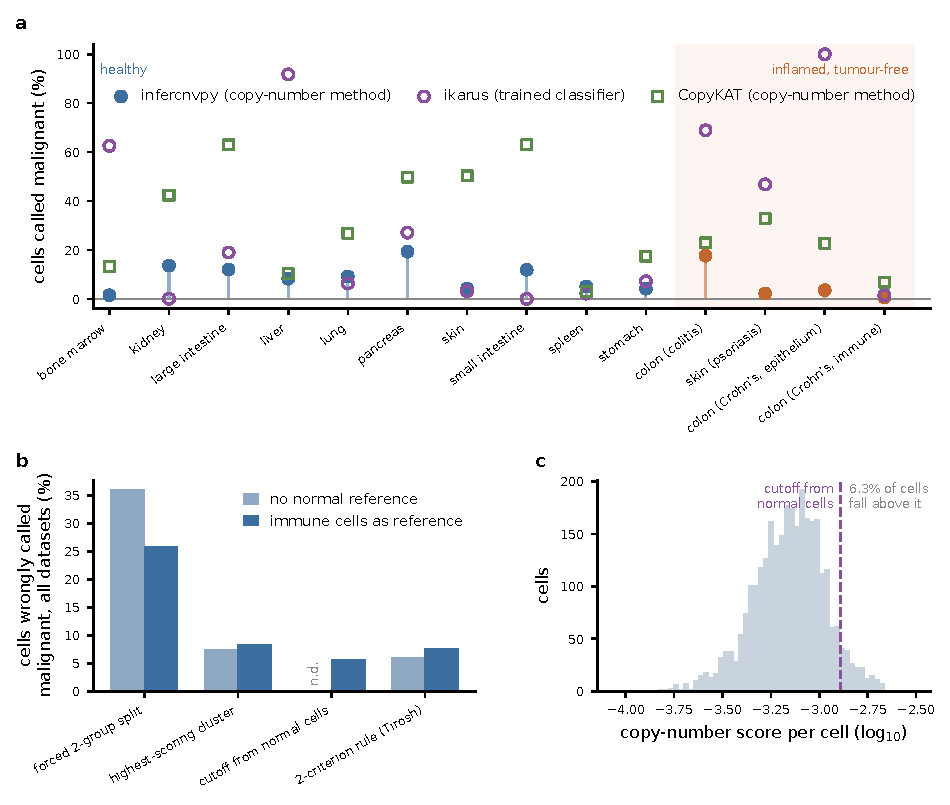
\includegraphics[width=0.95\textwidth]{Fig1_false_positives.pdf}
\caption{\textbf{Malignant-cell callers assign tumour labels to tumour-free tissue.}
\textbf{(a)} Percentage of cells called malignant in each of 14 tumour-free datasets by infercnvpy under the two-criterion (Tirosh) rule (filled circles), by CopyKAT (squares) and by ikarus (open circles). Every call shown is a false positive. The shaded region marks datasets from inflammatory-disease cohorts. infercnvpy values use the immune-reference mode where immune cells were available and the reference-free mode otherwise (Crohn's epithelium). Values are listed in Table~\ref{tab:panel}.
\textbf{(b)} False-call rate pooled over the panel (weighted by dataset size) for four decision rules applied to the same infercnvpy profiles, in reference-free and immune-reference modes. The reference-SD rule is undefined without a reference (n.d.).
\textbf{(c)} Distribution of the per-cell copy-number score in healthy lung (immune-reference mode; $n = 3{,}002$ cells). The dashed line is the reference-SD cutoff realized on this dataset. It falls inside the bulk of the distribution and calls 6.3\% of cells. The distribution appears unimodal, so any cut selects a tail of a continuous distribution rather than a separate population.}
\label{fig:fp}
\end{figure}

\begin{table}[htbp]
\centering
\caption{\textbf{Tumour-free panel and false malignant-call rates.} Every call is a false positive by construction. infercnvpy columns give the percentage of cells called malignant by infercnvpy under the two-criterion (Tirosh) rule and the forced two-group split, using the immune reference where one was available ($^{\dagger}$reference-free mode: no immune cells in the Crohn's epithelial dataset). CopyKAT was run on a cell-type-proportional subsample ($n$ shown); the aneuploid percentage uses all submitted cells as the denominator, with \texttt{not.defined} cells counted as not aneuploid. Pooled rates are weighted by dataset size. The pooled donor count is a sum over datasets; Tabula Sapiens donors contribute to several organs and the two Crohn's datasets come from one cohort, so it overstates the number of unique donors. Rates for all rules and both reference modes are in Supplementary Table~S1.}
\label{tab:panel}
\scriptsize
\setlength{\tabcolsep}{3.2pt}
\begin{tabular}{@{}llrrrrrrrrr@{}}
\toprule
 & & & & & \multicolumn{2}{c}{infercnvpy (\%)} & \multicolumn{3}{c}{CopyKAT} & ikarus \\
\cmidrule(lr){6-7}\cmidrule(lr){8-10}\cmidrule(lr){11-11}
Dataset & Assay & Cells & Donors & Types & Tirosh & Two-group & Aneu.\ (\%) & n.d.\ (\%) & $n$ & Tumour (\%) \\
\midrule
Bone marrow & 10x 3$'$ v3 & 3,003 & 5 & 18 & 1.5 & 23.5 & 13.3 & 1.0 & 1,206 & 62.5 \\
Kidney & 10x 3$'$ v3 & 1,315 & 1 & 8 & 13.6 & 15.0 & 42.4 & 0.0 & 1,198 & 0.0 \\
Large intestine & 10x 3$'$ v3 & 3,005 & 5 & 24 & 12.0 & 47.0 & 63.0 & 0.2 & 1,196 & 18.9 \\
Liver & 10x 3$'$ v3 & 2,995 & 4 & 20 & 8.2 & 4.3 & 10.3 & 3.5 & 1,186 & 91.8 \\
Lung & 10x 3$'$ v3 & 3,002 & 4 & 28 & 9.2 & 56.2 & 26.8 & 0.8 & 1,192 & 6.3 \\
Pancreas & 10x 3$'$ v3 & 1,887 & 3 & 13 & 19.3 & 19.6 & 49.8 & 0.7 & 1,204 & 27.1 \\
Skin & 10x 3$'$ v3 & 2,301 & 4 & 14 & 4.1 & 8.7 & 50.3 & 1.5 & 1,198 & 3.1 \\
Small intestine & 10x 3$'$ v3 & 2,995 & 5 & 29 & 11.9 & 37.2 & 63.0 & 0.2 & 1,192 & 0.0 \\
Spleen & 10x 3$'$ v3 & 2,997 & 6 & 21 & 5.1 & 22.5 & 3.0 & 3.6 & 1,210 & 2.2 \\
Stomach & 10x 3$'$ v3 & 2,995 & 3 & 18 & 4.2 & 6.5 & 17.4 & 2.7 & 1,200 & 7.2 \\
\midrule
Colon (UC cohort) & 10x 3$'$ v1 & 1,782 & 10 & 13 & 17.6 & 50.0 & 22.9 & 56.4 & 1,196 & 68.9 \\
Skin (psoriasis) & 10x 3$'$ v3 & 2,992 & 6 & 20 & 2.2 & 10.8 & 32.8 & 8.0 & 1,194 & 46.8 \\
Colon (Crohn's, epithelial) & 10x 3$'$ v2 & 2,249 & 10 & 7 & 3.6$^{\dagger}$ & 51.1$^{\dagger}$ & 22.7 & 43.0 & 591 & 100.0 \\
Colon (Crohn's, immune) & 10x 3$'$ v2 & 3,010 & 10 & 17 & 0.5 & 32.8 & 6.8 & 80.6 & 1,126 & 1.5 \\
\midrule
\textbf{Pooled} &  & 36,528 & 76 &  & 7.3 & 27.5 & 30.7 & 13.1 & 16,089 & 30.6 \\
\bottomrule
\end{tabular}
\end{table}


\subsection{Positive controls: what the callers can detect}

A false-positive rate can only be interpreted alongside the sensitivity it buys. Because tumour-free tissue contains no positives, we constructed them. From each of three healthy tissues (liver, lung and spleen) we drew 840 cells at random and imposed arm-level dosage changes of known burden. For each cell we sampled whole chromosome arms and scaled the counts of every gene on the affected arms up or down before re-normalisation. Each tissue received 120 cells at each of seven burdens (1, 2, 3, 5, 8, 12 and 18 arm-level events), 2{,}520 altered cells in total. These were scored together with 6{,}474 untouched diploid companion cells from the same samples, giving 8{,}994 cells. The altered cells are real cells in every respect except for a known, controlled karyotype. Within a tissue, all 120 cells at a given burden share one randomly drawn karyotype, so each burden is represented by three karyotypes in total; the non-monotone curves in Figure~\ref{fig:spike}a (for example spleen at 12 versus 18 events) partly reflect which arms were drawn.

Per-cell discrimination is weak at low burden and moderate at high burden (Figure~\ref{fig:spike}a; Supplementary Table~\ref{tab:s2}). In reference-free mode, the area under the ROC curve for separating altered from diploid cells with the continuous copy-number score averages 0.53 across tissues for a single arm event (0.50--0.57 per tissue), close to chance. It is 0.65 at five events and 0.85 at 18; immune-reference values are similar (0.53 to 0.83). This bounds what any threshold on this score can achieve, and the bound is modest: in these data, cells with five or fewer arm-level changes (mean AUC $\le 0.65$) are poorly separated from diploid cells by the infercnvpy score.

ikarus does not respond to dosage (Figure~\ref{fig:spike}b; Supplementary Table~\ref{tab:s3}). In each tissue, its call rate on cells carrying 12--18 events matches its call rate on the diploid companions: 80.0\% versus 83.2\% in liver, 3.3\% versus 6.3\% in lung, and 2.9\% versus 3.1\% in spleen. Its calls track the tissue context, which is consistent with its 100\% rate on Crohn's colonic epithelium and its 0\% rate on healthy kidney and small intestine. CopyKAT's response differs by tissue. In spleen it calls 58.3\% of diploid companions and 94.9\% of cells carrying 12--18 events aneuploid. In lung the corresponding rates are 14.9\% and 0.0\% (0 of 90 high-burden cells): the cells with the largest imposed karyotypes are the ones least likely to be called. In liver they are 1.7\% and 0.0\% (0 of 106), a difference that the small CopyKAT subsample cannot resolve. In no tissue other than spleen did CopyKAT's call rate rise with burden. CopyKAT emits a categorical call rather than a per-cell score, so it cannot enter the matched comparison below.

The comparison that matters in practice holds each method at the same false-call rate (Figure~\ref{fig:spike}c; Table~\ref{tab:matched}). For each rule and tissue, we measured the rule's false-call rate on diploid companions and its detection rate on cells carrying 12--18 events. We then thresholded the continuous score at exactly that false-call rate and recorded its detection rate. The matched threshold is a quantile of the score among the same diploid companions on which the false-call rate was measured, so the score is evaluated at an operating point chosen with knowledge of which cells are diploid, whereas the rules are not. The ratios below are therefore an upper bound on what a threshold can achieve, attainable only where a tumour-free reference of the query tissue is available --- which is what we recommend below. We included ikarus in this comparison as an external benchmark, although it is a separate classifier rather than a rule applied to the infercnvpy profile. In all 11 comparisons where a matched threshold could be evaluated, the score detected more altered cells than the rule or classifier. For the eight comparisons involving published rules on the infercnvpy profile the factor was 2.2--5.3; including the external classifier the full range is 1.2--10.3. The extremes of that wider range fall at operating points no analyst would adopt: the smallest factor (1.2) is the liver comparison with ikarus, matched at an 83.2\% false-call rate, and three of the 11 comparisons are matched above 20\% false calls (83.2\%, 56.4\% and 22.2\%). Setting those three aside, the factor over the remaining comparisons, all matched at 7\% false calls or below, is 2.2--10.3, and the score still wins every one (Table~\ref{tab:matched} lists the matched false-call rate of each). For the two-criterion rule the factor was 3.9--5.3 (for example 33.3\% versus 6.2\% in lung, both at 5.3\% false calls). The one comparison that could not be made favours the rule. In spleen, the highest-scoring-cluster rule detected 31.2\% of high-burden cells with no false calls among 2{,}157 diploid companions, and no score threshold at zero false calls was evaluated. With that exception, the published rules do not appear to extract information beyond the score; rather, they select a poor operating point on it. The two-criterion rule barely discriminates at all in this setting: its detection rate on cells with 12--18 events (4.6--6.2\%) is about the same as its false-call rate on diploid cells (4.5--6.5\%).

\begin{figure}[htbp]
\centering
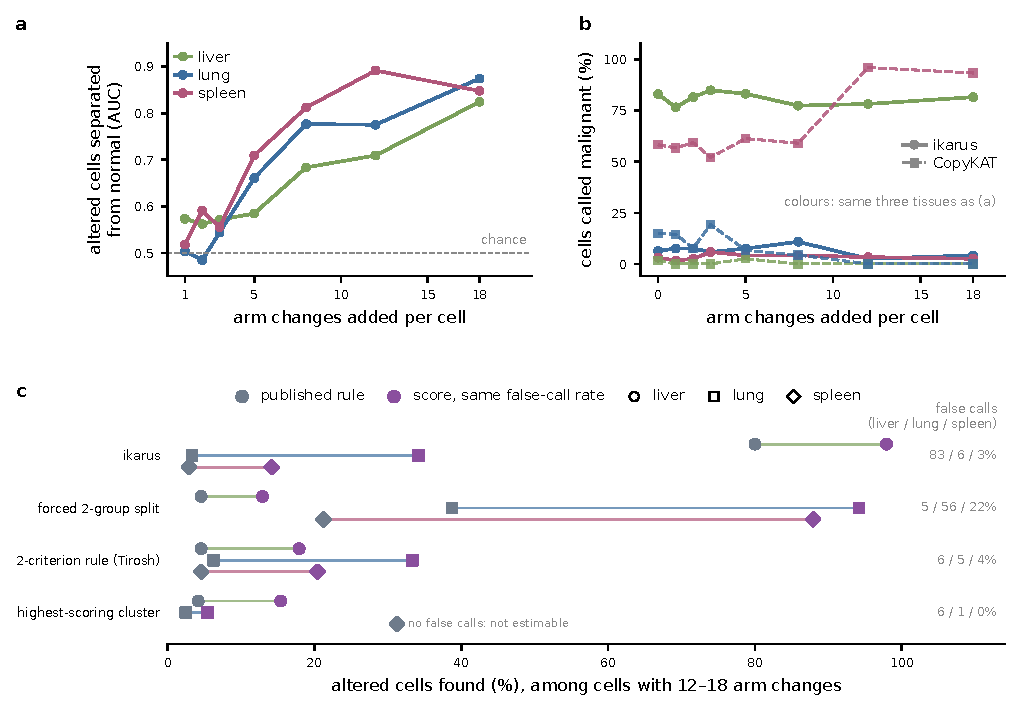
\includegraphics[width=0.95\textwidth]{Fig2_spikein.pdf}
\caption{\textbf{In-silico positive controls bound what the callers can detect.}
\textbf{(a)} Area under the ROC curve (AUC; 0.5 = chance) for separating altered from diploid cells using the continuous infercnvpy score (reference-free mode), by number of arm-level events imposed, in three tissues. Each point compares 120 altered cells with the 2{,}155--2{,}162 diploid companions of that tissue.
\textbf{(b)} Percentage of cells called malignant by ikarus (solid) and CopyKAT (dashed) by imposed burden; burden 0 denotes untouched diploid cells from the same sample. ikarus does not respond to dosage. CopyKAT responds in spleen only, and in liver and lung it calls the highest-burden cells least often.
\textbf{(c)} Detection of altered cells carrying 12--18 arm events, per tissue (marker shape), comparing each published rule (grey) with a threshold on the continuous score placed at exactly that rule's false-call rate on diploid companions (purple). Numbers at right give each rule's false-call rate in liver, lung and spleen. For the highest-scoring-cluster rule in spleen, the rule made no false calls and no matched score threshold was evaluated. Values are listed in Table~\ref{tab:matched}.}
\label{fig:spike}
\end{figure}

\begin{table}[htbp]
\centering
\caption{\textbf{Detection at matched false-call rate, per spike-in tissue.} For each rule, its false-call rate on diploid companion cells and its detection rate on cells carrying 12--18 arm events, compared with a threshold on the continuous infercnvpy score placed at exactly that false-call rate. The threshold is a quantile of the score among the same diploid companions used to measure the rule's false-call rate, so the ratios are an upper bound attainable only where such a reference exists. n.e.: not estimable; the rule made no false calls on spleen diploid cells, so no score threshold at 0\% false calls was evaluated.}
\label{tab:matched}
\small
\begin{tabular}{@{}llrrrr@{}}
\toprule
 & & False-call & \multicolumn{2}{c}{Detection, 12--18 events (\%)} & \\
\cmidrule(lr){4-5}
Rule & Tissue & rate (\%) & Rule & Score & Ratio \\
\midrule
Two-criterion (Tirosh) & Liver & 6.5 & 4.6 & 17.9 & 3.9$\times$ \\
Two-criterion (Tirosh) & Lung & 5.3 & 6.2 & 33.3 & 5.3$\times$ \\
Two-criterion (Tirosh) & Spleen & 4.5 & 4.6 & 20.4 & 4.5$\times$ \\
\addlinespace
Highest-scoring cluster & Liver & 5.8 & 4.2 & 15.4 & 3.7$\times$ \\
Highest-scoring cluster & Lung & 1.2 & 2.5 & 5.4 & 2.2$\times$ \\
Highest-scoring cluster & Spleen & 0.0 & 31.2 & n.e. & -- \\
\addlinespace
Forced two-group split & Liver & 5.0 & 4.6 & 12.9 & 2.8$\times$ \\
Forced two-group split & Lung & 56.4 & 38.8 & 94.2 & 2.4$\times$ \\
Forced two-group split & Spleen & 22.2 & 21.2 & 87.9 & 4.1$\times$ \\
\addlinespace
ikarus & Liver & 83.2 & 80.0 & 97.9 & 1.2$\times$ \\
ikarus & Lung & 6.3 & 3.3 & 34.2 & 10.3$\times$ \\
ikarus & Spleen & 3.1 & 2.9 & 14.2 & 4.9$\times$ \\
\bottomrule
\end{tabular}
\end{table}


\subsection{The false calls share a gene-density-driven pseudo-karyotype}

If false calls were random, the problem would be one of statistical power alone. They are not random. For the two-criterion rule (reference-free mode), we compared the mean inferred copy-number profile of falsely called cells with that of uncalled cells in each dataset, in 10-Mb genomic bins (Figure~\ref{fig:mech}a). The resulting difference profile is structured, with recurrent apparent losses and gains at specific loci. The strongest bins are an apparent gain at chr7:110--120 Mb and apparent losses at chr12:50--60 Mb and chr19:0--10 Mb. A reader would naturally interpret such a pattern as a shared clonal event.

The profile recurs across tissues that share no biology. Bin-level difference profiles of different datasets correlate with a median Spearman $\rho$ of 0.54 over all 91 dataset pairs (Figure~\ref{fig:mech}c; Supplementary Table~\ref{tab:s5}). Excluding the Crohn's immune dataset, per-dataset medians range from 0.24 (ulcerative colitis cohort) to 0.66. A genuine clonal event cannot be shared by healthy kidney, healthy spleen and psoriatic skin. One dataset is a clear exception. The Crohn's immune profile is anti-correlated with every other dataset ($\rho$ from $-0.49$ to $-0.11$), which indicates that the direction of the artefact can invert, at least in this dataset composed entirely of immune cells. We return to this in the Discussion.

The panel-averaged profile is predicted by local gene density (Figure~\ref{fig:mech}b). Across 278 genomic bins, the apparent copy-number shift correlates negatively with the number of genes in the bin (Spearman $\rho = -0.53$): gene-dense regions look deleted and gene-poor regions look gained. The three strongest bins illustrate the gradient directly --- the two apparent losses at chr19:0--10 Mb and chr12:50--60 Mb contain 630 and 544 genes, whereas the apparent gain at chr7:110--120 Mb contains 148.

Adjacent 10-Mb bins share smoothed windows, so they are not independent and the asymptotic $P$-value for this correlation ($2\times10^{-21}$) is not a calibrated test. We therefore re-tested the association against a null that preserves genomic autocorrelation, circularly shifting the binned profile within each chromosome relative to the gene counts (10{,}000 shifts). Autocorrelation alone does induce a negative correlation: the shift null is centred at $\rho = -0.21$ (s.d.\ 0.058) rather than at zero, so roughly 40\% of the observed coefficient is attributable to the bin structure itself. The observed $\rho = -0.53$ nonetheless lies 5.6 null standard deviations beyond that centre and was not reached by any of the 10{,}000 shifts (most extreme shift $\rho = -0.41$), giving $P < 10^{-4}$. The association therefore survives a test that respects the dependence between bins. Its size is the more informative quantity, and the association is consistent with a compositional artefact. Sliding-window averaging of library-size-normalised expression makes each window's value depend on relative rather than absolute expression. Cells whose expression distribution is broader or narrower than the reference --- because of cell state, RNA content or capture efficiency --- would therefore acquire a smooth, genome-wide, gene-density-dependent deviation. Such a deviation would survive the smoothing steps of copy-number callers, and because cells with similar technical properties share it, it would cluster those cells and make them resemble a clone. This mechanism is an interpretation; we did not test it directly, for example by perturbing library composition in silico. We also asked whether clustered gene families (immunoglobulin, T-cell receptor, HLA, histone, keratin and other locus-restricted families) explain the profile. They do not account for it as a class. Of the 278 bins, 85 overlap the locus of at least one of the 156 clustered families resolved at this bin size, and their mean absolute difference is 0.0011 \emph{lower} than that of the remaining bins (background mean 0.0076), against a shift null centred at $+0.0005$ (s.d.\ 0.0008); the same within-chromosome circular-shift procedure gives $P = 0.98$ for the hypothesis that family bins carry more signal. Individual family loci nonetheless appear among the strongest bins: the apparent loss at chr12:50--60 Mb coincides with both the type II keratin cluster and the \textit{HOXC} cluster, and reaches 4.2 times the background mean. Clustered families are therefore not the general explanation for the pseudo-karyotype, although particular loci contribute to it.

\begin{figure}[htbp]
\centering
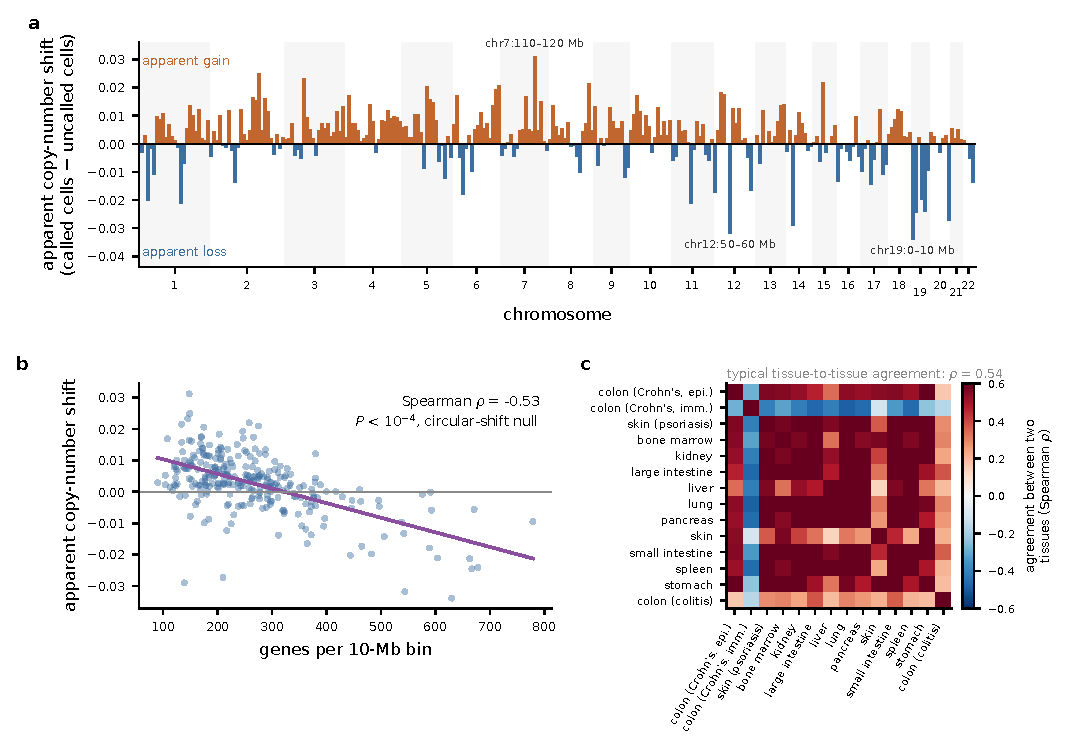
\includegraphics[width=0.95\textwidth]{Fig3_mechanism.pdf}
\caption{\textbf{False calls share a recurrent, gene-density-driven pseudo-karyotype.} A pseudo-karyotype is a chromosome-level pattern of apparent gains and losses with no clonal basis. Called cells are those called malignant by the two-criterion rule in reference-free mode.
\textbf{(a)} Mean inferred copy-number difference between falsely called and uncalled cells, in 10-Mb bins, averaged over datasets with at least 20 called cells. Labels mark the three strongest bins.
\textbf{(b)} Apparent copy-number shift against the number of genes per 10-Mb bin ($n = 278$ bins), with linear fit. Gene-dense regions look deleted. The quoted $P$ is from a within-chromosome circular-shift null (10{,}000 shifts), which preserves the autocorrelation between neighbouring bins; the asymptotic $P$-value for the same coefficient, $2\times10^{-21}$, assumes independence that does not hold.
\textbf{(c)} Spearman correlation between the bin-level difference profiles of each pair of datasets. Agreement across unrelated tissues indicates a technical rather than clonal origin. The Crohn's immune dataset is the exception and is anti-correlated with all others.}
\label{fig:mech}
\end{figure}

\subsection{An empirical-null decision rule reduces false calls about 90-fold}

The preceding results show that the score carries usable but limited dosage information and that published rules use it poorly. We therefore replaced the decision step and left the score unchanged (Methods). The procedure takes any per-cell score. It residualises the score on sequencing depth within each cell type, because the score depends on depth and cell types differ in depth. It then fits an empirical null distribution of the adjusted score on tumour-free reference cells of the same cell type. Each query cell receives a right-tail $p$-value against the null for its type; the extreme tail is extrapolated with a generalized Pareto fit~\cite{knijnenburg2009}. Cells are called aneuploid if they pass Benjamini--Hochberg (BH) control at level $\alpha$ within each sample~\cite{bh1995}; whether a sample was a dataset or a donor was not recorded, so we evaluate both cases. The procedure does not modify the caller.

On tumour-free data every call is a false discovery, so BH at level $\alpha$ makes two predictions if the $p$-values are valid. The per-cell false-call rate should be far below $\alpha$. More stringently, each BH family should receive any call at all with probability at most $\alpha$. Over the 13 datasets this bounds the expected number of datasets with any call at $13\alpha$ if each dataset is one family, or at $\sum_i \min(1, \alpha d_i)$ if each of the $d_i$ donors of dataset $i$ is a family. We tested both by leave-one-tissue-out validation, fitting the null on the healthy datasets other than the query dataset (Figure~\ref{fig:cal}; Table~\ref{tab:cal}; Supplementary Table~\ref{tab:s4}).

The first prediction holds in 13 of 14 datasets. At $\alpha = 5\%$ the per-cell false-call rate had a median of 0.03\% and a maximum of 0.43\% (lung), compared with 0.5--19.3\% for the two-criterion rule on the same cells (Figure~\ref{fig:cal}c). Across these 13 datasets the procedure made 28 false calls among 33{,}536 cells, against about 2{,}600 for the two-criterion rule. This reduction holds over the full range $\alpha = 1$--$10\%$ (Figure~\ref{fig:cal}a). A rule that calls almost nothing will trivially score well on tumour-free data, so this comparison establishes specificity only; we did not apply the calibrated rule to the spike-in cells, and its sensitivity relative to the published rules remains to be measured. The second prediction does not hold under either grouping. At $\alpha = 5\%$, 7 of the 13 datasets received at least one call (1 to 13 cells per dataset; Figure~\ref{fig:cal}b). The bound allows at most 0.65 such datasets on average with per-dataset BH and at most 3.5 with per-donor BH. Treating datasets as independent, 7 or more would occur with probability at most $1\times10^{-6}$ and 0.03, respectively; at $\alpha = 1\%$ (4 datasets against bounds of 0.13 and 0.70) the corresponding probabilities are $7\times10^{-6}$ and 0.004. The $p$-values are therefore anti-conservative for a small number of cells in the extreme tail, whether through the tail extrapolation, residual differences between the reference tissues and the query tissue, or both; and the procedure should be read as a large, verifiable reduction in false calls, not as exact error control.

Cell-type labels are not always available, so we also implemented a label-free variant. It assigns each cell to the nearest of a set of transcriptional archetypes derived from reference centroids and conditions on the archetype instead of the label. At $\alpha \le 5\%$ it made almost no calls in these 13 datasets: only one received any call (a single lung cell), consistent with both bounds. At $\alpha = 10\%$ it failed abruptly in two datasets, calling 18.2\% of Crohn's immune cells and 4.2\% of liver cells, and on psoriatic skin it called no cells at $\alpha \le 2\%$ but 57.0\% at $\alpha = 5\%$ (Supplementary Table~\ref{tab:s4}). This all-or-nothing pattern is characteristic of BH once a block of $p$-values falls below its threshold. The label-free variant should therefore be used only at strict levels, and only with a null that transfers to the query.

The single dataset in which the cell-type-conditioned procedure failed is informative. On psoriatic skin, the null fitted on the Tabula Sapiens tissues gave a per-cell false-call rate of 26.8\% at $\alpha = 5\%$, higher than the 2.2\% of the two-criterion rule it replaces. This failure occurred even though the reference included healthy skin. The dataset uses the same 10x 3$'$ v3 chemistry as the reference tissues but comes from a different study, laboratory and disease state. Conversely, the Crohn's (v2) and ulcerative colitis (v1) datasets differ in chemistry yet were controlled (0--0.07\%). Chemistry alone therefore does not explain transferability. Being from a separate study is not sufficient either, since the Crohn's and colitis datasets transferred well; our data do not identify the cause. In a separate donor-held-out evaluation (Figure~\ref{fig:cal}d; Table~\ref{tab:cal}), a null fitted on the other donors of the same dataset reduced the psoriasis rate from 27.1\% to 0.03\%, with a maximum of 3.67\% (liver) across the 13 eligible datasets. This evaluation was run separately from the leave-one-tissue-out analysis, and because it is restricted to donors contributing at least 200 cells it does not always score the same cells: its cell count is lower than the leave-one-tissue-out count for 7 of the 13 datasets (for example 837 versus 1{,}782 cells for the colitis cohort and 2{,}874 versus 2{,}997 for spleen). Its cross-tissue arm agrees with the leave-one-tissue-out rate to within 0.01 percentage points for 8 of the 13 datasets and to within 0.4 points for two more (psoriatic skin 0.37, spleen 0.39). Three datasets disagree substantially, and for all three the two arms score an identical set of cells, so the difference is not one of cell selection: large intestine (3.83\% versus 0.00\%, $n = 3{,}005$ in both), liver (4.31\% versus 0.00\%, $n = 2{,}995$) and lung (1.00\% versus 0.43\%, $n = 3{,}002$). We report both as computed (Limitations). The same-dataset null was not uniformly better: in liver it still called 3.67\% of cells, and in the ulcerative colitis and small-intestine datasets it called slightly more cells than the cross-tissue null (0.12\% versus 0.00\% and 0.03\% versus 0.00\%). The evidence that same-study nulls are preferable therefore rests mainly on psoriatic skin. Our practical recommendation is that the null should be drawn from cells processed like the query cells, and that the realized false-call rate of any null should be checked on held-out tumour-free cells before use.

\begin{figure}[htbp]
\centering
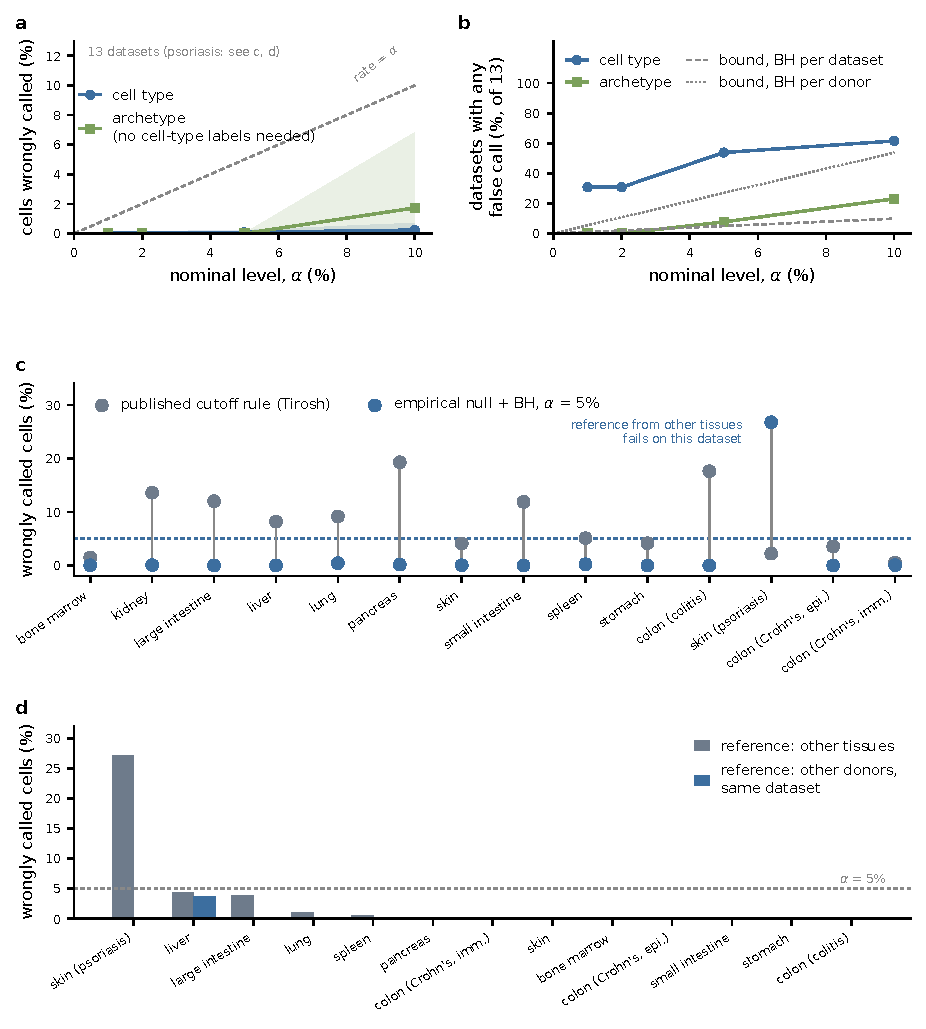
\includegraphics[width=0.95\textwidth]{Fig4_calibration.pdf}
\caption{\textbf{An empirical-null decision rule reduces false calls but is not exactly calibrated in the extreme tail.}
\textbf{(a)} Per-cell false-call rate against nominal BH level $\alpha$ under leave-one-tissue-out validation, for nulls conditioned on annotated cell type (blue) or on label-free archetype (green). Mean $\pm$ s.d.\ across 13 datasets (psoriatic skin shown in c and d). The dashed line marks rate $= \alpha$. Because every call on tumour-free data is a false discovery, BH predicts a per-cell rate far below this line.
\textbf{(b)} Percentage of the 13 datasets that received at least one call. With valid $p$-values, BH bounds the probability of any call by $\alpha$ per family; lines show the resulting bound on this percentage if BH is applied per dataset (dashed) or per donor (dotted). The cell-type-conditioned procedure exceeds both bounds at every level up to 5\%.
\textbf{(c)} False-call rate per dataset for the two-criterion rule (grey; reference mode as in Figure~\ref{fig:fp}a) and for the cell-type-conditioned procedure at $\alpha = 5\%$ (blue). The horizontal dotted line marks the nominal level $\alpha = 5\%$; on tumour-free data every call is a false discovery, so a valid procedure should fall far below it.
\textbf{(d)} Separate donor-held-out evaluation at $\alpha = 5\%$: a null fitted on other tissues (grey) versus one fitted on held-out donors of the same dataset (blue), on cells of donors contributing at least 200 cells. It scores fewer cells than panel (c) for 7 of 13 datasets, and its cross-tissue arm does not match panel (c) for three datasets whose cell sets are identical (see text and Table~\ref{tab:cal}).}
\label{fig:cal}
\end{figure}

\begin{table}[htbp]
\centering
\caption{\textbf{Calibrated decision rule at nominal level $\alpha = 5\%$.} Tirosh: false-call rate of the two-criterion rule (as in Table~\ref{tab:panel}). Leave-one-tissue-out (LOTO): null fitted on the healthy datasets other than the query, conditioned on annotated cell type (false calls / cells, per-cell false-call rate and Wilson 95\% interval) or on label-free archetype. Donor-held-out: a separate evaluation on cells of donors with at least 200 cells, comparing a null from other tissues with a null from the other donors of the same dataset. Because of that restriction its denominator is smaller than the LOTO denominator for 7 of 13 datasets, so the two sets of columns do not always score the same cells; where they do, its cross-tissue column still fails to reproduce the LOTO column for three datasets (large intestine, liver, lung; see Limitations). --: dataset not eligible (fewer than two qualifying donors).}
\label{tab:cal}
\scriptsize
\setlength{\tabcolsep}{3.5pt}
\begin{tabular}{@{}lrrrrrrr@{}}
\toprule
 & & \multicolumn{4}{c}{LOTO null (\%)} & \multicolumn{2}{c}{Donor-held-out (\%)} \\
\cmidrule(lr){3-6}\cmidrule(lr){7-8}
Dataset & Tirosh (\%) & Calls & Rate & 95\% CI & Archetype & Other tissues & Same dataset \\
\midrule
Bone marrow & 1.5 & 1/3,003 & 0.03 & 0.01--0.19 & 0.00 & 0.03 & 0.03 \\
Kidney & 13.6 & 1/1,315 & 0.08 & 0.01--0.43 & 0.00 & -- & -- \\
Large intestine & 12.0 & 0/3,005 & 0.00 & 0.00--0.13 & 0.00 & 3.83 & 0.03 \\
Liver & 8.2 & 0/2,995 & 0.00 & 0.00--0.13 & 0.00 & 4.31 & 3.67 \\
Lung & 9.2 & 13/3,002 & 0.43 & 0.25--0.74 & 0.03 & 1.00 & 0.00 \\
Pancreas & 19.3 & 3/1,887 & 0.16 & 0.05--0.47 & 0.00 & 0.16 & 0.00 \\
Skin & 4.1 & 1/2,301 & 0.04 & 0.01--0.25 & 0.00 & 0.04 & 0.00 \\
Small intestine & 11.9 & 0/2,995 & 0.00 & 0.00--0.13 & 0.00 & 0.00 & 0.03 \\
Spleen & 5.1 & 7/2,997 & 0.23 & 0.11--0.48 & 0.00 & 0.63 & 0.03 \\
Stomach & 4.2 & 0/2,995 & 0.00 & 0.00--0.13 & 0.00 & 0.00 & 0.00 \\
\midrule
Colon (UC cohort) & 17.6 & 0/1,782 & 0.00 & 0.00--0.22 & 0.00 & 0.00 & 0.12 \\
Skin (psoriasis) & 2.2 & 801/2,992 & 26.77 & 25.22--28.39 & 56.99 & 27.14 & 0.03 \\
Colon (Crohn's, epithelial) & 3.6 & 0/2,249 & 0.00 & 0.00--0.17 & 0.00 & 0.00 & 0.00 \\
Colon (Crohn's, immune) & 0.5 & 2/3,010 & 0.07 & 0.02--0.24 & 0.00 & 0.07 & 0.00 \\
\bottomrule
\end{tabular}
\end{table}


% ---------- Section: Discussion ----------
\section{Discussion}

We ran three widely used malignant-cell callers on 14 tumour-free datasets, where every positive call is false. Under published decision rules they called up to 19.3\% (two-criterion rule), 63.0\% (CopyKAT) and 100\% (ikarus) of cells malignant. In-silico positive controls showed that the underlying copy-number score separates altered from diploid cells only moderately, and that the rules use it at poor operating points. The false calls carried a recurrent pseudo-karyotype that tracks gene density. An empirical-null decision layer reduced false calls about 90-fold but did not achieve exact error control, and it failed in one dataset, psoriatic skin from a separate study, when the null was drawn from Tabula Sapiens tissues that included healthy skin; two other datasets from separate studies were controlled.

These rates contrast with the accuracy reported when the callers were introduced. CopyKAT distinguished cancer cells from normal cell types with 98\% accuracy across 21 tumours~\cite{copykat}, ikarus was reported to achieve high sensitivity and specificity~\cite{ikarus}, and SCEVAN to discriminate malignant from non-malignant cells accurately~\cite{scevan}. Those evaluations were made on tumour samples, where a population of truly aneuploid cells exists for a binary split or a tumour-trained classifier to find. Our panel asks what happens when there is nothing to find. A forced two-group split, which CopyKAT's classification resembles, must still return a malignant group. A supervised classifier must still place each cell on one side of a boundary learned from tumour data, and ikarus placed whole tissues on the tumour side (100\% of Crohn's colonic epithelium, 91.8\% of healthy liver). Our results agree with a recent comparison in endometrial cancer, which found that CopyKAT and SCEVAN substantially overestimated the number of tumour cells, and that inferCNV score distributions did not clearly separate malignant from non-malignant populations~\cite{dugo2025}. The unimodal score we observed in healthy lung is the tumour-free counterpart of that observation.

Two recent independent benchmarks evaluated copy-number callers against orthogonal DNA-based ground truth in tumours~\cite{schmid2025,song2025}. Schmid and colleagues found that performance depended on dataset-specific factors, including the choice of reference dataset, and that methods using allelic information were more robust on large droplet-based datasets~\cite{schmid2025}. Song and colleagues found that Numbat performed best across most criteria and that CopyKAT performed best when only an expression matrix was available. They also assessed aneuploidy calls among non-malignant cells within tumours~\cite{song2025}. Our results are consistent with both studies and extend them in two directions. First, reference choice mattered here as well: the immune-reference and reference-free modes gave different false-call rates for the same rule, and a null drawn from other tissues failed on psoriatic skin while one drawn from the same study did not. Second, we show that the decision rule applied after inference contributes to false calls, independently of the inference algorithm: the same profiles gave pooled false-call rates that differed up to six-fold between rules. Allele-aware methods were not tested here, and the benchmarks above suggest they may be less affected.

Our design assumes that essentially all cells in tumour-free tissue are euploid. Direct single-cell DNA sequencing of mouse and human tissues supports this: aneuploidy is rare, including in liver and brain, where high frequencies had previously been reported, and is no more prevalent there than in skin~\cite{knouse2014}. Clonal copy-number changes in non-malignant tissue therefore cannot account for false-call rates of tens of per cent, such as 63.0\% of healthy intestinal cells by CopyKAT or 91.8\% of healthy liver cells by ikarus.

The pseudo-karyotype we observed connects to an earlier observation. When HoneyBADGER combined allelic and expression signals in tumours, prominent transcriptional subpopulations did not line up with the genetic subclones and were likely driven by nonclonal mechanisms~\cite{honeybadger}. Our results give a concrete example of how this can arise from expression alone. The difference profile of falsely called cells correlates with local gene density and recurs across unrelated tissues, so it cannot reflect a shared clone. It is the kind of structured, reproducible signal that clonal analyses are designed to detect. Because this artefact is a property of expression composition, allele-based evidence~\cite{honeybadger,numbat} should provide an independent check on it, although we have not tested this directly.

The calibration layer follows an established statistical idea. Efron argued that in large-scale testing the null distribution should often be estimated from the data rather than assumed~\cite{efron2004}; we estimate it from tumour-free reference cells of the same cell type. Apart from the depth adjustment, which is fitted on the same reference cells, $p$-values computed by ranking a query cell's score among reference scores are conformal $p$-values. Bates and colleagues showed that such $p$-values are marginally valid and positively dependent, so that Benjamini--Hochberg control of the false-discovery rate holds across them (in a marginal sense, averaged over the reference set), provided reference and query cells are exchangeable~\cite{bates2023}. This framework is consistent with our main observations. Psoriatic skin from a separate study plausibly departs from exchangeability with Tabula Sapiens reference cells, and the procedure failed there. A null drawn from held-out donors of the same dataset comes closer to exchangeability, and false calls in psoriatic skin fell from 27.1\% to 0.03\%. The residual false calls in 7 of 13 datasets may reflect smaller departures from exchangeability or the generalized Pareto extrapolation~\cite{knijnenburg2009}, which extends $p$-values below the $1/(n+1)$ floor of the empirical null but is not covered by the conformal guarantee. The practical consequence is that the reference set matters as much as the statistical procedure, and the realized false-call rate should be verified rather than assumed.

These findings support several practical recommendations. Report a false-positive rate, measured on tumour-free cells processed like the query, alongside any malignant compartment. Prefer the continuous score to a binary label where the downstream analysis permits. Where a label is required, set the threshold from an explicit null drawn from comparable cells, and verify the realized rate. Treat an apparent shared karyotype among called cells as a warning sign, and check it against gene density before interpreting it as clonal. Where allelic information is available, use it as an independent check.

% ---------- Section: Limitations ----------
\section{Limitations}

This study was executed at a reduced scale relative to its design, and several reductions are material.

\textbf{Panel size and sampling.} Each dataset was subsampled to approximately 3{,}000 cells, so that the full set of callers, reference modes and decision rules could be run on a single workstation. Per-dataset rates therefore carry sampling uncertainty (Wilson intervals for the calibrated rule are given in Table~\ref{tab:cal}). Each analysis was run on one subsample with one random seed; we did not repeat subsampling. Pooled rates are more stable than individual ones.

\textbf{Callers covered.} We ran infercnvpy rather than the original R implementation of inferCNV~\cite{infercnv}. infercnvpy implements the same sliding-window algorithm but is not bit-identical, so the rates reported here should not be attributed to the R package without verification. CopyKAT was run on a cell-type-proportional subsample of approximately 1{,}200 cells per dataset (591--1{,}210 cells; 16{,}089 in total) because of its single-threaded runtime, so its rates carry wider uncertainty. CopyKAT was also run in its default immune-reference configuration only, since it emits a categorical call rather than a score. Several callers in common use were not run: CONICSmat~\cite{conics}, SCEVAN~\cite{scevan}, Numbat~\cite{numbat} and other allele-aware methods~\cite{casper,honeybadger}. Allele-aware methods are of particular interest, because the artefact we describe is compositional and would not be expected to affect allelic imbalance in the same way. Benchmarks on tumour data suggest that these methods are more robust~\cite{schmid2025,song2025}. Testing them on tumour-free tissue is the most important extension of this audit.

\textbf{Positive controls are in silico.} The altered cells are real cells with simulated arm-level dosage changes, not tumour cells with karyotypes established by an orthogonal assay. The simulation imposes a clean multiplicative dosage effect and so probably overstates detectability relative to real tumour cells, where dosage compensation, subclonal structure and focal events complicate the signal. The AUC values should be read as upper bounds. The spike-in analysis covers three tissues and one karyotype per burden per tissue, so per-burden values reflect the particular arms drawn. AUC values are reported without confidence intervals; each rests on 120 altered cells against 2{,}155--2{,}162 diploid companions, which corresponds to a 95\% interval of roughly $\pm0.05$, so the ordering of adjacent burdens is not resolved by these data. In the matched comparison, the score's threshold is a quantile taken among the same diploid companions on which the false-call rate is measured, so that comparison is in-sample for the score and out-of-sample for the rules; the detection ratios are an upper bound rather than an estimate of practical gain.

\textbf{No matched orthogonal ground truth.} We did not analyse a dataset with matched single-cell DNA or bulk copy-number profiling. Such data would allow false-positive and false-negative rates to be measured on tumour tissue rather than inferred from tumour-free tissue and simulation~\cite{schmid2025,song2025}.

\textbf{Composition of the inflammatory-cohort datasets.} Of the four non-healthy datasets, three contain cells annotated as diseased. The fourth (colon, ulcerative colitis cohort) contains only cells annotated as non-diseased from that cohort. Conclusions about inflammation as a driver of false calls rest on the former three.

\textbf{Calibration analysis.} Leave-one-tissue-out validation used tumour-free tissue only. It therefore measures false calls, not the false-discovery rate in the presence of true positives, and it does not measure sensitivity. The calibrated rule could have been applied to the spike-in cells but was not; until it is, its gain in specificity cannot be weighed against any loss of sensitivity. Query cell types absent from the reference (for example hepatocytes when liver is held out) are scored against the pooled null, so the conditioning on cell type is incomplete for tissue-specific types. The Poisson-binomial tail probabilities treat datasets as independent, although Tabula Sapiens organs share donors and the two Crohn's datasets share a cohort. The grouping used for BH (whole dataset or donor) was not recorded; we therefore test the excess of datasets with any call against the bound implied by each grouping, and the conclusion holds under both for $\alpha \le 5\%$. The probabilities quoted for that excess treat datasets as independent and use the bound itself as each dataset's probability, which makes them conservative. The donor-held-out evaluation was restricted to datasets with at least two donors contributing at least 200 cells each, so for 7 of 13 datasets it scores fewer cells than the leave-one-tissue-out analysis. It was run separately from that analysis, and for three datasets whose two arms score an identical set of cells (large intestine, liver and lung) its cross-tissue arm does not reproduce the leave-one-tissue-out rate. The cause cannot be determined from the retained outputs.

\textbf{Reproducibility.} All figures and tables can be regenerated from the released summary results. Some upstream components, however, were not retained in reusable form: the step that aggregates per-cell caller output into summary results, the chromosome-arm boundaries used for the spike-ins, and the Ensembl release used for gene coordinates. Because the per-cell scores of the spike-in cells were not retained either, the sensitivity analysis noted above could not be added without re-running that arm of the pipeline, which would not reproduce the published values exactly. These components will be restored in a revised version.

% ---------- Section: Methods ----------
\section{Methods}

\subsection{Data}

Healthy tissues were obtained from the Tabula Sapiens atlas~\cite{tabula} through CZ CELLxGENE Discover~\cite{cellxgene2025}, selecting primary 10x 3$'$ v3 data from adult donors. Inflammatory-cohort datasets were obtained from the same source~\cite{kong2023,gao2021pso,smillie2019}. Within each dataset, cells from the dominant assay were retained and filtered to at least 500 UMIs, at least 250 detected genes and at most 50\% mitochondrial reads; the mitochondrial cap was deliberately lenient, because a stringent cap would preferentially remove mitochondria-rich epithelial cells, the types most at risk of false calls. Cell types with fewer than 40 cells were excluded. Up to 200 cells were then drawn at random from each combination of annotated cell type and disease status, and the result was downsampled proportionally to approximately 3{,}000 cells. Because the cap applies per disease status, datasets containing both diseased and non-diseased cells can contain more than 200 cells of one type (up to 400 in the Crohn's epithelial dataset). Sampling was not stratified by donor. Genes were restricted to those with an assigned chromosome and position in the annotation used by the callers. Per-dataset composition is summarised in Table~\ref{tab:panel}.

\subsection{Copy-number inference and classification}

infercnvpy 0.6.1~\cite{infercnvpy} was run on each dataset on log-normalised expression (total counts scaled to $10^4$, then $\log(1+x)$), with 100-gene sliding windows, a 10-gene step, log-fold-change clipping at 3 and a dynamic noise threshold of 1.5, in two modes. In reference-free mode no reference category was set. In immune-reference mode, cells whose annotated type matched a curated immune vocabulary by whole-word match (T, B, NK, plasma, myeloid, monocyte, macrophage, Kupffer, Langerhans, dendritic, mast, neutrophil and other granulocyte cells, and their subtypes) were designated the reference category; this mode required at least 50 immune cells and was therefore not run on the Crohn's epithelial dataset. The per-cell score used throughout is the mean squared deviation of the window profile.

CopyKAT 1.2.5~\cite{copykat} was run in R 4.4.3 with the same immune-reference designation and default parameters, on a per-dataset subsample of approximately 1{,}200 cells drawn proportionally across annotated cell types. Rates use all submitted cells as the denominator; cells returned as \texttt{not.defined} are reported separately.

ikarus 0.0.3~\cite{ikarus} was run with its published pan-cancer gene signatures and pretrained logistic-regression core model, unchanged, using AUCell scoring~\cite{aucell} followed by cell--cell network propagation over 100 nearest neighbours as implemented in the package (signature adaptation enabled). ikarus emits a hard tumour/normal label per cell and takes no reference.

\subsection{Decision rules}

Five rules were applied to the infercnvpy output. (R1) \emph{Forced two-group split}: Ward hierarchical clustering of the CNV profile (first 30 principal components) cut into two groups, with the group of higher mean score declared malignant; this mirrors the binary split made by CopyKAT and cannot return `no tumour'. (R1b) \emph{Highest-scoring cluster}: Leiden clustering~\cite{leiden} of the CNV profile at resolution 1.0, with the single highest-mean-score cluster declared malignant. (R2) \emph{Per-cell quantile}: cells above the 90th percentile of the per-cell score declared malignant; this rule calls 10\% of cells by construction and is not tabulated. (R3) \emph{Reference SD}: cells whose score exceeds the reference-cell mean by more than three reference standard deviations; this rule requires a reference. (R4) \emph{Two-criterion (Tirosh)}~\cite{tirosh2016,tirosh2016b,puram2017}: cells whose score exceeds the reference mean by more than two reference standard deviations and whose CNV profile correlates above 0.4 with the mean profile of the top-scoring 5\% of cells (at least 10 cells). In reference-free mode the lowest-scoring 20\% of cells serve as the reference for the score threshold.

\subsection{In-silico aneuploid spike-ins}

For each of three healthy tissues (liver, lung and spleen), 840 cells were drawn at random without replacement and split into seven groups of 120, one per burden $b \in \{1, 2, 3, 5, 8, 12, 18\}$. Each group received one karyotype of $b$ chromosome arms drawn without replacement (acrocentric short arms excluded), each designated a loss (copy number 1) or a gain with equal probability; gains were copy number 3, or 4 with probability 0.15. UMI counts of genes on affected arms were binomially thinned (losses) or augmented (gains) to the target dosage ratio, and each cell's total count was then restored to its original value by binomial resampling, so that each altered cell keeps the depth of a real cell but has an altered relative expression profile. Untouched cells from the same tissue served as diploid companions. Truth labels and burdens were withheld from all scoring. Discrimination was summarised by the ROC AUC of the per-cell score for altered versus diploid cells at each burden. For the matched comparison, each rule's false-call rate on diploid companions was computed, the score threshold yielding the same false-call rate on the same diploid cells was found, and detection rates on cells with 12--18 events were compared.

\subsection{Empirical-null decision rule}

Let $s_i$ be the per-cell copy-number score and $d_i$ the log total count. Within each reference cell type $t$ with at least 40 cells, $s$ is regressed linearly on $d$; types with fewer cells use a pooled regression. The residual $r_i = s_i - \hat{s}_t(d_i)$ is retained. The null for type $t$ is the empirical distribution of $r$ over reference cells of that type, for types with at least 100 reference cells; other types, including query types absent from the reference, use the pooled null. A query cell of type $t$ receives the right-tail empirical $p$-value $p_i = (1 + \#\{r \in F_t : r \ge r_i\}) / (n_t + 1)$. Beyond the 90th percentile of the null, $p_i$ is replaced by a generalized Pareto tail estimate~\cite{knijnenburg2009}, provided the Pareto fit is not rejected by an Anderson--Darling test ($P > 0.05$) and at least 50 exceedances are available. Cells are called aneuploid if their BH-adjusted $q$-value~\cite{bh1995}, computed within each sample, is at most $\alpha$. The label-free variant replaces $t$ with the archetype whose reference centroid correlates best with the cell; centroids are mean log-normalised profiles of reference cell types with at least 50 cells, restricted to the 2{,}000 genes most variable across centroids.

In leave-one-tissue-out validation the null was fitted on all healthy tissues except the query dataset and then applied to the query dataset, at $\alpha \in \{1, 2, 5, 10\}\%$. We report the per-cell false-call rate with a Wilson 95\% interval~\cite{wilson1927}, and the number of datasets with at least one call. That number was compared with its BH bound under per-dataset grouping (each dataset receives a call with probability at most $\alpha$) and under per-donor grouping (at most $\min(1, \alpha d_i)$ for a dataset with $d_i$ donors), using the exact upper tail of the Poisson-binomial distribution with those probabilities. The donor-held-out evaluation fitted the null on all donors of a dataset except one and applied it to the held-out donor, cycling over donors contributing at least 200 cells.

\subsection{Attribution analysis}

For each dataset with at least 20 cells called by the two-criterion rule (reference-free mode), the difference profile was computed as the mean window value of called cells minus that of uncalled cells, aggregated into 10-Mb bins containing at least five windows. Gene counts per bin were taken from the annotation used by the caller. The panel-averaged profile is the unweighted mean over all 14 per-dataset profiles, including the Crohn's immune dataset whose profile is anti-correlated with the others; averaging it in with the same sign attenuates rather than inflates the association, which is $\rho = -0.51$ when that dataset is excluded. Gene density was related to the panel-averaged profile by Spearman correlation. Because neighbouring bins are autocorrelated, the asymptotic $P$-value is reported for completeness rather than as a calibrated test, and significance was assessed instead against a circular-shift null: the binned profile was shifted circularly within each chromosome by an independent random offset, leaving the gene counts in place, and the Spearman correlation recomputed (10{,}000 shifts, seed 0). This preserves the autocorrelation of the profile and the gene-count distribution while breaking their positional correspondence. The reported $P$ is the proportion of shifts whose correlation was at least as extreme as the observed one, with the usual $(1 + \#)/(1 + N)$ correction. Cross-tissue reproducibility was quantified as the Spearman correlation between bin-level difference profiles of each pair of datasets, over bins present in at least six datasets. Clustered gene families were tested by comparing the mean absolute difference in bins overlapping family loci with that of other bins, using the same within-chromosome circular-shift null (2{,}000 shifts, seed 0) applied to the binned absolute difference.

\subsection{Statistical analysis}

Associations between continuous quantities were assessed by Spearman rank correlation. Where the quantities were indexed along the genome and therefore autocorrelated, significance was assessed against a within-chromosome circular-shift null rather than an asymptotic $P$-value (Attribution analysis). Discrimination between altered and diploid cells was summarised by the area under the receiver operating characteristic curve. Pooled false-call rates are cell-weighted averages across datasets, and per-dataset proportions are reported with Wilson 95\% confidence intervals~\cite{wilson1927}. The number of datasets receiving at least one call under the calibrated rule was compared with its Benjamini--Hochberg bound using exact Poisson-binomial tail probabilities, as described above.

\subsection{Software}

Analyses were performed in Python 3 using scanpy~\cite{scanpy}, anndata, NumPy, SciPy and scikit-learn, together with infercnvpy (v0.6.1) and ikarus (v0.0.3), and in R (v4.4.3) using CopyKAT (v1.2.5). Figures were prepared with matplotlib (v3.11.1).

\subsection{Data availability}

All datasets analysed in this study are publicly available through CZ CELLxGENE Discover~\cite{cellxgene2025}. The ten healthy-organ datasets are from Tabula Sapiens~\cite{tabula}. The inflammatory-disease datasets are from published studies of Crohn's disease~\cite{kong2023}, psoriasis~\cite{gao2021pso} and ulcerative colitis~\cite{smillie2019}. The CELLxGENE dataset identifier for each of the 14 panel datasets, together with its assay, its cell count as downloaded and its cell count after filtering and subsampling, is given in Supplementary Table~\ref{tab:s6}. No new data were generated by this study. The result tables underlying every figure, table and number in this manuscript are released with the analysis code (\texttt{results/T0--T10}, including the test statistics for the gene-density and gene-family comparisons in \texttt{T6b}, \texttt{T9b} and \texttt{T9c}).

% ---------- Back Matter ----------
\section*{Code availability}
All analysis code, result tables, figure and table scripts are available at \url{https://github.com/hossainlab/sc-cnv-fps}.

\section*{Author contributions}
CRediT roles. \textbf{Md. Jubayer Hossain:} conceptualization, methodology, software, formal analysis, investigation, data curation, visualization, writing --- original draft, writing --- review and editing, project administration. \textbf{Preonath Chondrow Dev:} conceptualization, methodology, validation, investigation, writing --- review and editing. Both authors had full access to the result tables underlying every reported number, approved the submitted version, and accept responsibility for the decision to submit.

\section*{Competing interests}
The authors declare no competing interests.

\section*{Use of AI tools}
AI-assisted tools (Claude Science) were used to support data analysis, figure preparation, manuscript writing and critical review of the manuscript, under the direction of the authors. The authors reviewed and verified all outputs and take full responsibility for the analysis, its interpretation and the content of this manuscript.

\section*{Funding}
This work received no specific funding.

% ---------- References ----------
\renewcommand{\bibfont}{\small}
\bibliographystyle{unsrtnat}
\bibliography{scCNV-FP-Evaluation}

% ---------- Supplementary ----------
\clearpage
\suppfloats
\section*{Supplementary Information}
\addcontentsline{toc}{section}{Supplementary Information}

Supplementary Tables~S1--S6 report the full results underlying the main figures and tables, and the provenance of the panel datasets.

\begin{table}[htbp]
\centering
\caption{\textbf{False malignant-call rate (\%) of infercnvpy under four published decision rules and two reference modes.} The per-cell quantile rule (90th percentile) is omitted because it calls 10\% of cells by construction. n.d.: the reference-SD rule is undefined without a reference. n.a.: no immune reference cells available. Pooled rates are weighted by dataset size over the datasets where the rule is defined.}
\label{tab:s1}
\scriptsize
\begin{tabular}{@{}llrrrr@{}}
\toprule
Dataset & Mode & Two-group & Top cluster & Ref.\ SD & Tirosh \\
\midrule
Bone marrow & Reference-free & 23.2 & 0.8 & n.d. & 11.9 \\
Bone marrow & Immune reference & 23.5 & 0.3 & 0.3 & 1.5 \\
Kidney & Reference-free & 14.9 & 7.4 & n.d. & 4.0 \\
Kidney & Immune reference & 15.0 & 18.9 & 11.2 & 13.6 \\
Large intestine & Reference-free & 30.9 & 1.3 & n.d. & 6.1 \\
Large intestine & Immune reference & 47.0 & 16.2 & 6.2 & 12.0 \\
Liver & Reference-free & 4.5 & 5.5 & n.d. & 6.6 \\
Liver & Immune reference & 4.3 & 5.6 & 9.8 & 8.2 \\
Lung & Reference-free & 56.4 & 0.4 & n.d. & 5.7 \\
Lung & Immune reference & 56.2 & 0.3 & 6.3 & 9.2 \\
Pancreas & Reference-free & 16.0 & 7.0 & n.d. & 14.9 \\
Pancreas & Immune reference & 19.6 & 8.9 & 16.5 & 19.3 \\
Skin & Reference-free & 8.7 & 8.3 & n.d. & 9.3 \\
Skin & Immune reference & 8.7 & 8.3 & 1.0 & 4.1 \\
Small intestine & Reference-free & 69.8 & 1.4 & n.d. & 3.4 \\
Small intestine & Immune reference & 37.2 & 1.2 & 8.1 & 11.9 \\
Spleen & Reference-free & 22.5 & 5.1 & n.d. & 5.9 \\
Spleen & Immune reference & 22.5 & 5.2 & 2.5 & 5.1 \\
Stomach & Reference-free & 19.1 & 5.6 & n.d. & 6.0 \\
Stomach & Immune reference & 6.5 & 4.8 & 3.3 & 4.2 \\
Colon (UC cohort) & Reference-free & 71.0 & 8.0 & n.d. & 2.5 \\
Colon (UC cohort) & Immune reference & 50.0 & 10.7 & 12.1 & 17.6 \\
Skin (psoriasis) & Reference-free & 78.0 & 19.3 & n.d. & 0.9 \\
Skin (psoriasis) & Immune reference & 10.8 & 14.0 & 4.5 & 2.2 \\
Colon (Crohn's, epithelial) & Reference-free & 51.1 & 16.1 & n.d. & 3.6 \\
Colon (Crohn's, epithelial) & Immune reference & n.a. & n.a. & n.a. & n.a. \\
Colon (Crohn's, immune) & Reference-free & 30.0 & 21.0 & n.d. & 5.5 \\
Colon (Crohn's, immune) & Immune reference & 32.8 & 21.1 & 0.5 & 0.5 \\
\textbf{Pooled} & Reference-free & 36.0 & 7.5 & n.d. & 6.1 \\
\textbf{Pooled} & Immune reference & 25.9 & 8.4 & 5.7 & 7.6 \\
\bottomrule
\end{tabular}
\end{table}

\begin{table}[htbp]
\centering
\caption{\textbf{Per-cell discrimination of in-silico aneuploid cells from diploid companions.} Area under the ROC curve for the continuous infercnvpy score (mean squared deviation of the window profile) by number of imposed arm-level events. Each entry compares 120 aneuploid cells with the 2,155--2,162 untouched diploid companions of the same tissue (2,520 aneuploid and 6,474 diploid cells in total).}
\label{tab:s2}
\scriptsize
\begin{tabular}{@{}llrrrrrrr@{}}
\toprule
 & & \multicolumn{7}{c}{Arm-level events per cell} \\
\cmidrule(lr){3-9}
Mode & Tissue & 1 & 2 & 3 & 5 & 8 & 12 & 18 \\
\midrule
Reference-free & Liver & 0.57 & 0.56 & 0.57 & 0.58 & 0.68 & 0.71 & 0.82 \\
Reference-free & Lung & 0.50 & 0.48 & 0.54 & 0.66 & 0.78 & 0.78 & 0.87 \\
Reference-free & Spleen & 0.52 & 0.59 & 0.56 & 0.71 & 0.81 & 0.89 & 0.85 \\
Reference-free & \textit{Mean} & \textit{0.53} & \textit{0.55} & \textit{0.56} & \textit{0.65} & \textit{0.76} & \textit{0.79} & \textit{0.85} \\
\midrule
Immune reference & Liver & 0.57 & 0.57 & 0.56 & 0.56 & 0.66 & 0.69 & 0.82 \\
Immune reference & Lung & 0.51 & 0.49 & 0.56 & 0.64 & 0.76 & 0.72 & 0.84 \\
Immune reference & Spleen & 0.52 & 0.59 & 0.55 & 0.70 & 0.80 & 0.88 & 0.82 \\
Immune reference & \textit{Mean} & \textit{0.53} & \textit{0.55} & \textit{0.56} & \textit{0.63} & \textit{0.74} & \textit{0.76} & \textit{0.83} \\
\bottomrule
\end{tabular}
\end{table}

\begin{table}[htbp]
\centering
\caption{\textbf{Response of ikarus and CopyKAT to imposed karyotype burden.} Percentage of cells called tumour (ikarus) or aneuploid (CopyKAT); burden 0 denotes untouched diploid companion cells. ikarus was applied to all cells (6,474 diploid, 120 per burden per tissue); CopyKAT to a subsample (cell counts shown).}
\label{tab:s3}
\scriptsize
\begin{tabular}{@{}llrrrrrrrr@{}}
\toprule
Tissue & Caller & 0 & 1 & 2 & 3 & 5 & 8 & 12 & 18 \\
\midrule
Liver & ikarus & 83.2 & 76.7 & 81.7 & 85.0 & 83.3 & 77.5 & 78.3 & 81.7 \\
 & CopyKAT & 1.7 & 0.0 & 0.0 & 0.0 & 2.5 & 0.0 & 0.0 & 0.0 \\
 & \quad CopyKAT $n$ & 866 & 42 & 28 & 56 & 40 & 48 & 58 & 48 \\
Lung & ikarus & 6.3 & 7.5 & 7.5 & 5.8 & 7.5 & 10.8 & 2.5 & 4.2 \\
 & CopyKAT & 14.9 & 14.5 & 7.7 & 19.2 & 6.7 & 4.3 & 0.0 & 0.0 \\
 & \quad CopyKAT $n$ & 886 & 62 & 26 & 52 & 30 & 46 & 58 & 32 \\
Spleen & ikarus & 3.1 & 1.7 & 2.5 & 5.8 & 4.2 & 4.2 & 3.3 & 2.5 \\
 & CopyKAT & 58.3 & 56.8 & 59.4 & 52.2 & 61.4 & 59.1 & 96.2 & 93.5 \\
 & \quad CopyKAT $n$ & 902 & 44 & 32 & 46 & 44 & 44 & 52 & 46 \\
\bottomrule
\end{tabular}
\end{table}

\begin{table}[htbp]
\centering
\caption{\textbf{Realized per-cell false-call rate (\%) of the calibrated rule across nominal levels.} Leave-one-tissue-out null conditioned on cell type or on label-free archetype. The last row of each block counts datasets, excluding psoriatic skin, with at least one false call. Under Benjamini--Hochberg control at level $\alpha$ with valid $p$-values, the expected count is at most $13\alpha$ if each dataset is one BH family, or $\sum_i \min(1, \alpha d_i) = 0.70, 1.40, 3.50, 7.00$ at the four levels if each of the $d_i$ donors of dataset $i$ is a family.}
\label{tab:s4}
\scriptsize
\begin{tabular}{@{}llrrrr@{}}
\toprule
Conditioning & Dataset & $\alpha=1\%$ & $\alpha=2\%$ & $\alpha=5\%$ & $\alpha=10\%$ \\
\midrule
Cell type & Bone marrow & 0.00 & 0.00 & 0.03 & 0.03 \\
 & Kidney & 0.08 & 0.08 & 0.08 & 0.08 \\
 & Large intestine & 0.00 & 0.00 & 0.00 & 0.00 \\
 & Liver & 0.00 & 0.00 & 0.00 & 1.67 \\
 & Lung & 0.30 & 0.30 & 0.43 & 0.47 \\
 & Pancreas & 0.11 & 0.11 & 0.16 & 0.16 \\
 & Skin & 0.00 & 0.00 & 0.04 & 0.04 \\
 & Small intestine & 0.00 & 0.00 & 0.00 & 0.00 \\
 & Spleen & 0.10 & 0.13 & 0.23 & 0.53 \\
 & Stomach & 0.00 & 0.00 & 0.00 & 0.00 \\
 & Colon (UC cohort) & 0.00 & 0.00 & 0.00 & 0.00 \\
 & Skin (psoriasis) & 2.84 & 11.20 & 26.77 & 44.82 \\
 & Colon (Crohn's, epithelial) & 0.00 & 0.00 & 0.00 & 0.00 \\
 & Colon (Crohn's, immune) & 0.00 & 0.00 & 0.07 & 0.07 \\
 & \textit{Datasets with $\geq$1 call (of 13)} & \textit{4} & \textit{4} & \textit{7} & \textit{8} \\
\midrule
Archetype & Bone marrow & 0.00 & 0.00 & 0.00 & 0.00 \\
 & Kidney & 0.00 & 0.00 & 0.00 & 0.00 \\
 & Large intestine & 0.00 & 0.00 & 0.00 & 0.00 \\
 & Liver & 0.00 & 0.00 & 0.00 & 4.24 \\
 & Lung & 0.00 & 0.00 & 0.03 & 0.03 \\
 & Pancreas & 0.00 & 0.00 & 0.00 & 0.00 \\
 & Skin & 0.00 & 0.00 & 0.00 & 0.00 \\
 & Small intestine & 0.00 & 0.00 & 0.00 & 0.00 \\
 & Spleen & 0.00 & 0.00 & 0.00 & 0.00 \\
 & Stomach & 0.00 & 0.00 & 0.00 & 0.00 \\
 & Colon (UC cohort) & 0.00 & 0.00 & 0.00 & 0.00 \\
 & Skin (psoriasis) & 0.00 & 0.00 & 56.99 & 70.82 \\
 & Colon (Crohn's, epithelial) & 0.00 & 0.00 & 0.00 & 0.00 \\
 & Colon (Crohn's, immune) & 0.00 & 0.00 & 0.00 & 18.21 \\
 & \textit{Datasets with $\geq$1 call (of 13)} & \textit{0} & \textit{0} & \textit{1} & \textit{3} \\
\bottomrule
\end{tabular}
\end{table}

\begin{table}[htbp]
\centering
\caption{\textbf{Reproducibility of the false-call difference profile.} Median Spearman correlation of each dataset's 10-Mb-bin difference profile (falsely called minus uncalled cells, two-criterion rule, reference-free mode) with those of the other 13 datasets. The Crohn's immune profile is anti-correlated with every other dataset (Spearman $\rho$ from -0.49 to -0.11).}
\label{tab:s5}
\small
\begin{tabular}{@{}lrr@{}}
\toprule
Dataset & Median $\rho$ & Donors \\
\midrule
Bone marrow & 0.56 & 5 \\
Kidney & 0.62 & 1 \\
Large intestine & 0.61 & 5 \\
Liver & 0.48 & 4 \\
Lung & 0.66 & 4 \\
Pancreas & 0.66 & 3 \\
Skin & 0.33 & 4 \\
Small intestine & 0.66 & 5 \\
Spleen & 0.61 & 6 \\
Stomach & 0.57 & 3 \\
Colon (UC cohort) & 0.24 & 10 \\
Skin (psoriasis) & 0.60 & 6 \\
Colon (Crohn's, epithelial) & 0.53 & 10 \\
Colon (Crohn's, immune) & -0.41 & 10 \\
\bottomrule
\end{tabular}
\end{table}

\begin{table}[htbp]
\centering
\caption{\textbf{Provenance of the 14 panel datasets.} Each dataset was obtained from CZ CELLxGENE Discover~\cite{cellxgene2025} as a single \texttt{.h5ad} file, retrievable at \url{https://datasets.cellxgene.cziscience.com/}\texttt{<dataset ID>}\texttt{.h5ad}. Source cells is the number of cells in the downloaded file; analysed cells is the number retained after restriction to the dominant assay, quality filtering, the per-cell-type cap and proportional downsampling (Methods). Dataset identifiers are also listed in \texttt{config/panel\_def.json} in the code repository.}
\label{tab:s6}
\scriptsize
\setlength{\tabcolsep}{4pt}
\begin{tabular}{@{}llrrll@{}}
\toprule
Dataset & Assay & Source cells & Analysed cells & CELLxGENE dataset ID & Study \\
\midrule
Bone marrow & 10x 3$'$ v3 & 27,112 & 3,003 & \texttt{4aedb645-7487-4ab0-ad95-ee4db1b8eccd} & \cite{tabula} \\
Kidney & 10x 3$'$ v3 & 11,376 & 1,315 & \texttt{76b6cf23-56db-4eac-8ee8-d84ce64c0395} & \cite{tabula} \\
Large intestine & 10x 3$'$ v3 & 30,084 & 3,005 & \texttt{81781bd2-7a71-43a8-ab31-2a9009c1aea6} & \cite{tabula} \\
Liver & 10x 3$'$ v3 & 22,214 & 2,995 & \texttt{a4b3a49e-062b-4e3f-8915-02f40607651f} & \cite{tabula} \\
Lung & 10x 3$'$ v3 & 65,847 & 3,002 & \texttt{fddf43a3-b7c8-49e9-ac0a-5e24b390849f} & \cite{tabula} \\
Pancreas & 10x 3$'$ v3 & 14,140 & 1,887 & \texttt{ba587dee-e050-4a31-bcb8-05e5418f9086} & \cite{tabula} \\
Skin & 10x 3$'$ v3 & 17,786 & 2,301 & \texttt{c240d5bc-a521-4330-a76b-7d566e939d87} & \cite{tabula} \\
Small intestine & 10x 3$'$ v3 & 42,036 & 2,995 & \texttt{6db4dfe6-d421-4287-a9dc-22eaa59be966} & \cite{tabula} \\
Spleen & 10x 3$'$ v3 & 70,448 & 2,997 & \texttt{5498457f-6a18-4766-b9a3-a2c8c4662703} & \cite{tabula} \\
Stomach & 10x 3$'$ v3 & 33,064 & 2,995 & \texttt{3e8bd2b2-fe53-4b95-abb2-ce971b4f1c14} & \cite{tabula} \\
\midrule
Colon (UC cohort) & 10x 3$'$ v1 & 34,772 & 1,782 & \texttt{774d77e7-210d-4237-8ca8-8d2bb841a2e4} & \cite{smillie2019} \\
Skin (psoriasis) & 10x 3$'$ v3 & 24,126 & 2,992 & \texttt{75eae05f-4f07-4518-a434-ea0a0d7ac616} & \cite{gao2021pso} \\
Colon (Crohn's, epithelial) & 10x 3$'$ v2 & 97,788 & 2,249 & \texttt{333491b4-ca9b-4369-8706-38f7bb5bcd46} & \cite{kong2023} \\
Colon (Crohn's, immune) & 10x 3$'$ v2 & 152,509 & 3,010 & \texttt{1ddca82d-2948-4dbe-8bba-be9de7115bb7} & \cite{kong2023} \\
\bottomrule
\end{tabular}
\end{table}


\end{document}
